\documentclass[tikz,border=0pt]{standalone}
\usepackage[utf8]{inputenc}
\usepackage[T1]{fontenc}
\usepackage{lmodern}
\usepackage{amsmath,amssymb}
\usetikzlibrary{arrows.meta,positioning,fit,calc,backgrounds,shapes.geometric,decorations.pathreplacing}
\definecolor{navy}{HTML}{163A5F}
\definecolor{blue}{HTML}{2C6EAF}
\definecolor{lightblue}{HTML}{EAF2F8}
\definecolor{midblue}{HTML}{CFE1F2}
\definecolor{graytext}{HTML}{4A5560}
\definecolor{lightgray}{HTML}{F4F6F8}
\definecolor{green}{HTML}{3C8D73}
\definecolor{lightgreen}{HTML}{E8F5EF}
\definecolor{red}{HTML}{B24A4A}
\definecolor{lightred}{HTML}{FBEDEE}
\tikzset{
  title/.style={font=\sffamily\bfseries\fontsize{16}{18}\selectfont,text=navy,anchor=west},
  subtitle/.style={font=\sffamily\bfseries\fontsize{11}{13}\selectfont,text=navy},
  body/.style={font=\sffamily\fontsize{9.2}{11}\selectfont,text=graytext,align=left},
  small/.style={font=\sffamily\fontsize{8}{9.4}\selectfont,text=graytext,align=left},
  tinylabel/.style={font=\sffamily\fontsize{7.2}{8.4}\selectfont,text=graytext},
  panel/.style={rounded corners=3pt,draw=midblue,fill=white,line width=0.6pt},
  box/.style={rounded corners=2pt,draw=midblue,fill=lightblue,line width=0.6pt},
  worker/.style={rounded corners=2pt,draw=blue,dashed,line width=0.7pt,fill=white},
  task/.style={rounded corners=2pt,draw=blue,fill=lightblue,minimum width=0.85cm,minimum height=0.55cm,font=\sffamily\bfseries\small,text=navy},
  file/.style={draw=blue,fill=white,minimum width=0.55cm,minimum height=0.42cm,font=\sffamily\small,text=navy},
  arr/.style={-{Stealth[length=2.4mm,width=1.8mm]},draw=blue,line width=0.9pt},
  arrthin/.style={-{Stealth[length=2mm,width=1.5mm]},draw=blue,line width=0.7pt},
  arrred/.style={-{Stealth[length=2mm,width=1.5mm]},draw=red,dashed,line width=0.8pt},
  arrgreen/.style={-{Stealth[length=2mm,width=1.5mm]},draw=green,dotted,line width=1pt}
}
\begin{document}

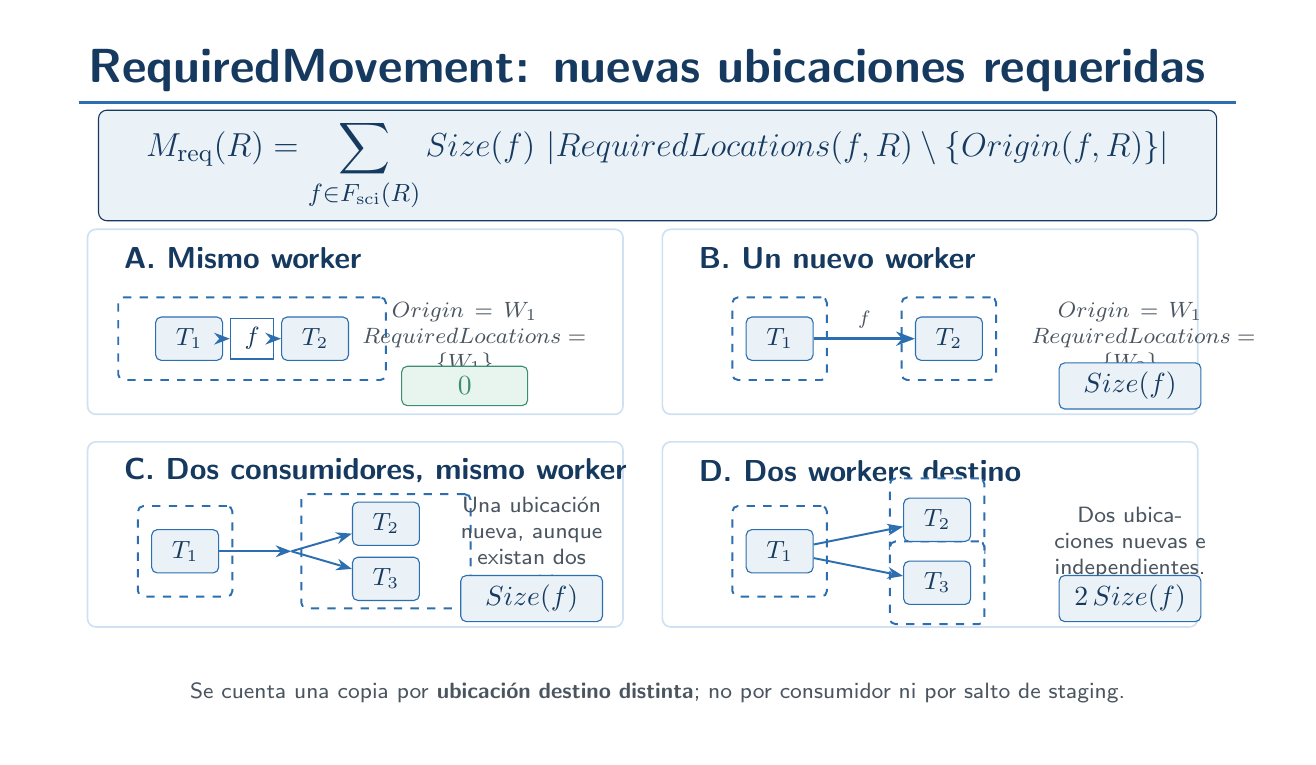
\begin{tikzpicture}[x=1cm,y=1cm]
\path[use as bounding box] (0,0) rectangle (16,9);
\node[title] at (0.65,8.45) {RequiredMovement: nuevas ubicaciones requeridas};
\draw[blue,line width=1pt] (0.65,8.05)--(15.35,8.05);
\node[rounded corners=3pt,draw=navy,fill=lightblue,minimum width=14.2cm,minimum height=1.05cm,font=\sffamily\bfseries\fontsize{13}{15}\selectfont,text=navy] at (8,7.25) {$M_{\mathrm{req}}(R)=\displaystyle\sum_{f\in F_{\mathrm{sci}}(R)} Size(f)\,\left|RequiredLocations(f,R)\setminus\{Origin(f,R)\}\right|$};

\foreach \x/\y/\ttl in {0.75/6.45/{A. Mismo worker},8.05/6.45/{B. Un nuevo worker},0.75/3.75/{C. Dos consumidores, mismo worker},8.05/3.75/{D. Dos workers destino}}{
\node[panel,minimum width=6.8cm,minimum height=2.35cm,anchor=north west] at (\x,\y) {};
\node[subtitle,anchor=west] at (\x+0.35,\y-0.38) {\ttl};
}
% A
\node[worker,minimum width=3.4cm,minimum height=1.05cm] at (2.85,5.05) {};
\node[task] (a1) at (2.05,5.05) {$T_1$}; \node[file] (af) at (2.85,5.05) {$f$}; \node[task] (a2) at (3.65,5.05) {$T_2$};
\draw[arrthin] (a1)--(af); \draw[arrthin] (af)--(a2);
\node[small,text width=2.6cm,align=center] at (5.55,5.05) {$Origin=W_1$\\$RequiredLocations=\{W_1\}$};
\node[rounded corners=2pt,draw=green,fill=lightgreen,font=\sffamily\bfseries,text=green,minimum width=1.6cm,minimum height=0.5cm] at (5.55,4.45) {$0$};
% B
\node[worker,minimum width=1.2cm,minimum height=1.05cm] at (9.55,5.05) {}; \node[worker,minimum width=1.2cm,minimum height=1.05cm] at (11.7,5.05) {};
\node[task] (b1) at (9.55,5.05) {$T_1$}; \node[task] (b2) at (11.7,5.05) {$T_2$};
\draw[arr] (b1)-- node[above,tinylabel] {$f$} (b2);
\node[small,text width=2.5cm,align=center] at (14.0,5.05) {$Origin=W_1$\\$RequiredLocations=\{W_2\}$};
\node[rounded corners=2pt,draw=blue,fill=lightblue,font=\sffamily\bfseries,text=navy,minimum width=1.8cm,minimum height=0.5cm] at (14.0,4.45) {$Size(f)$};
% C
\node[worker,minimum width=1.2cm,minimum height=1.15cm] at (2.0,2.35) {}; \node[worker,minimum width=2.15cm,minimum height=1.45cm] at (4.55,2.35) {};
\node[task] (c1) at (2.0,2.35) {$T_1$}; \node[task] (c2) at (4.55,2.7) {$T_2$}; \node[task] (c3) at (4.55,2.0) {$T_3$};
\draw[arrthin] (c1)--(3.35,2.35); \draw[arrthin] (3.35,2.35)--(c2); \draw[arrthin] (3.35,2.35)--(c3);
\node[small,text width=2.3cm,align=center] at (6.4,2.45) {Una ubicación nueva, aunque existan dos consumidores.};
\node[rounded corners=2pt,draw=blue,fill=lightblue,font=\sffamily\bfseries,text=navy,minimum width=1.8cm,minimum height=0.5cm] at (6.4,1.75) {$Size(f)$};
% D
\node[worker,minimum width=1.2cm,minimum height=1.15cm] at (9.55,2.35) {}; \node[worker,minimum width=1.2cm,minimum height=1.05cm] at (11.55,2.75) {}; \node[worker,minimum width=1.2cm,minimum height=1.05cm] at (11.55,1.95) {};
\node[task] (d1) at (9.55,2.35) {$T_1$}; \node[task] (d2) at (11.55,2.75) {$T_2$}; \node[task] (d3) at (11.55,1.95) {$T_3$};
\draw[arrthin] (d1)--(d2); \draw[arrthin] (d1)--(d3);
\node[small,text width=2.3cm,align=center] at (14.0,2.45) {Dos ubicaciones nuevas e independientes.};
\node[rounded corners=2pt,draw=blue,fill=lightblue,font=\sffamily\bfseries,text=navy,minimum width=1.8cm,minimum height=0.5cm] at (14.0,1.75) {$2\,Size(f)$};
\node[small,text width=14.2cm,align=center] at (8,0.55) {Se cuenta una copia por \textbf{ubicación destino distinta}; no por consumidor ni por salto de staging.};
\end{tikzpicture}
\end{document}
